\chapter{Parameters optimization}\label{optimization}
Code FAINA allows not only to evaluate radiation from the source, but also to fit model data to observations and obtain parameters of the source. There are various types optimization methods and models of loss functions, implemented in the code.

\section{Evaluators of the loss function}

The first thing one should determine to start optimization process is a loss function. In FAINA code abstract class LossEvalator and derived classes are used for it. All implemented classes use quadratic loss functions, taking into account observational errors:
$L = \sum \frac{(F_i - F_{obs,i})^2}{\sigma_i^2}$, where $F_i$ - is some modeled function of radiation (e.g. energy spectral density) evaluated at point corresponding to some observation, $F_{obs,i}$ - observed value of this function, $\sigma_i$ - it's uncertancy. There are following classes of loss function evaluator implemented in the cod: SpectrumLossEvaluator - for fitting energy flux spectral density in given time moment, TimeDependentSpectrumLossEvaluator - for fitting energy flux spectal density in different time moments and RadialProfileLossEvaluator - for fitting luminocity of the prolonged source in different points depending on radius in tangent plane. Public methods of this classes are listed in Table \ref{LossEvaluators}.

\begin{small}
	\topcaption{Public methods of loss function evaluators}
	\label{LossEvaluators}
	\begin{xtabular}{|p{0.5\textwidth}|p{0.5\textwidth}|}
		\hline
		\textbf{LossEvaluator} & абстрактный класс вычислителя целевой функции\\
		\hline
		virtual double evaluate(const double* vector, const double* maxParameters, RadiationEvaluator* evaluator) & чисто виртуальный метод, возвращающий значение целевой функции при данных параметрах. Так же на вход принимает вектор нормироваочных значений и вычислитель излучения\\
		\hline
		\textbf{SpectrumLossEvaluator} & класс, в котором целевая функция характеризует отличие вычисленной спектральной плотности излучения от наблюдательных данных, $f = \sum \frac{(F(E_i) - F_{obs,i})^2}{\sigma_i^2}$, где $F(E_i)$ - расчетная спектральная плотность потока излучения при данной энергии $E_i$, $F_{obs,i}$ - наблюдаемая спектральная плотность потока излучения, $\sigma_i$ - её погрешность.\\
		\hline
		SpectrumLossEvaluator(double* energy, double* observedFlux, double* observedError, int Ne, RadiationSource* radiatiornSource) & конструктор, принимает на вход наблюдаемые значения спектральной плотности энергии, их количество и источник, для которого нужно вычислять излучение \textcolor{red}{в каких единицах?}\\
		\hline
		\textbf{TimeDependentSpectrumLossEvaluator} & класс, в котором целевая функция характеризует отличие вычисленной спектральной плотности излучения от наблюдательных данных, собранных в различные моменты времени, $f = \sum \frac{(F(E_{ij}, t_j) - F_{obs,i,j})^2}{\sigma_{ij}^2}$, где $F(E_{ij},t_j)$ - расчетная спектральная плотность потока излучения при данной энергии $E_{ij}$ в момент времени $t_j$, $F_{obs,i,j}$ - наблюдаемая спектральная плотность потока излучения, $\sigma_{ij}$ - её погрешность. ОБРАТИТЕ ВНИМАНИЕ, что количество наблюдательных точек в разные моменты времени может быть разным\\
		\hline
		TimeDependentSpectrumLossEvaluator(double** energy, double** observedFlux, double** observedError, int* Ne, double* times, int Ntimes, RadiationTimeDependentSource* radiationSource) & конструктор, принимает на вход двумерные массиы наблюдаемых значений спектральной плотности энергии, массив количества точек в разные моменты времени и зависящий от времени источник, для которого нужно вычислять излучение \textcolor{red}{в каких единицах?}\\
		\hline
		\textbf{RadialProfileLossEvaluator} & класс, в котором целевая функция характеризует отличие радиальной зависимости яркости источника в заданном дипазоне от наблюдательных данных. $f = \sum \frac{(F(R_i) - F_{obs,i})^2}{\sigma_i^2}$, где $F(R_i)$ - расчетная яркость источника при данном радиусе $R_i$, $F_{obs,i}$ - наблюдаемая яркость, $\sigma_i$ - её погрешность\\
		\hline
		RadialProfileLossEvaluator(double energy, double* observedFlux, double* observedError, double* rhoPoints, int Nrho, RadiationSource* radiaionSource) & конструктор, принимающий на вход значение энергии, для которого нужно вычислять яркость, наблюдаемые потоки, погрешности и соответствующие значения радиуса, количество точек и источник, для которого нужно рассчитывать излучение\\
		\hline
	\end{xtabular}
\end{small}

\section{Оптимизаторы целевой функции}
Для фитирования постоянных во времени кривых блеска предназначен абстрактный класс RadiationOptimizer. В нем определена виртуальныя функция optimize(double* vector, bool* optPar), которая и производит процесс оптимизации. Входными параметрами являются: vector - массив подбираемых параметров, в который будет записан результат работы программы, optPar - массив булевских переменных, определяющих оптимизировать соответствующий параметр, или считать его фиксированным. Функция изменения параметров источника source->resetParameters, который будет использоваться в процессе оптимизации, описанная в разделе \ref{sourcesSection}, должна быть согласована с массивом оптимизируемых параметров vector, так как в процессе оптимизации он будет передаваться в нее в качестве аргумента.

В коде реализованы три наследника класса RadiationOptimazer: GridEnumRadiationOptimizer - производящий поиск минимума простым перебором по сетке параметров с заданным количеством распределенных равномерно логарифмически точек, GradientDescentRadiationOptimizer - в котором минимум находится методом градиентного спуска, и CombinedRadiationOptimizer, который выполняет оптимизацию двумя этими методами последовательно, используя результат работы первого как начальную точку для второго. Схема насследования классов оптимизаторов показана на рисунке \ref{radiationOptimizer}, а список их публичных методов приведен в Таблице \ref{RadiationOptimizerMethods}. Реализованные методы оптимизации применимы для всех описанных выше типов источников, видов электромагнитного излучения и вычислителей целевых функций.
\begin{figure}
	\centering
	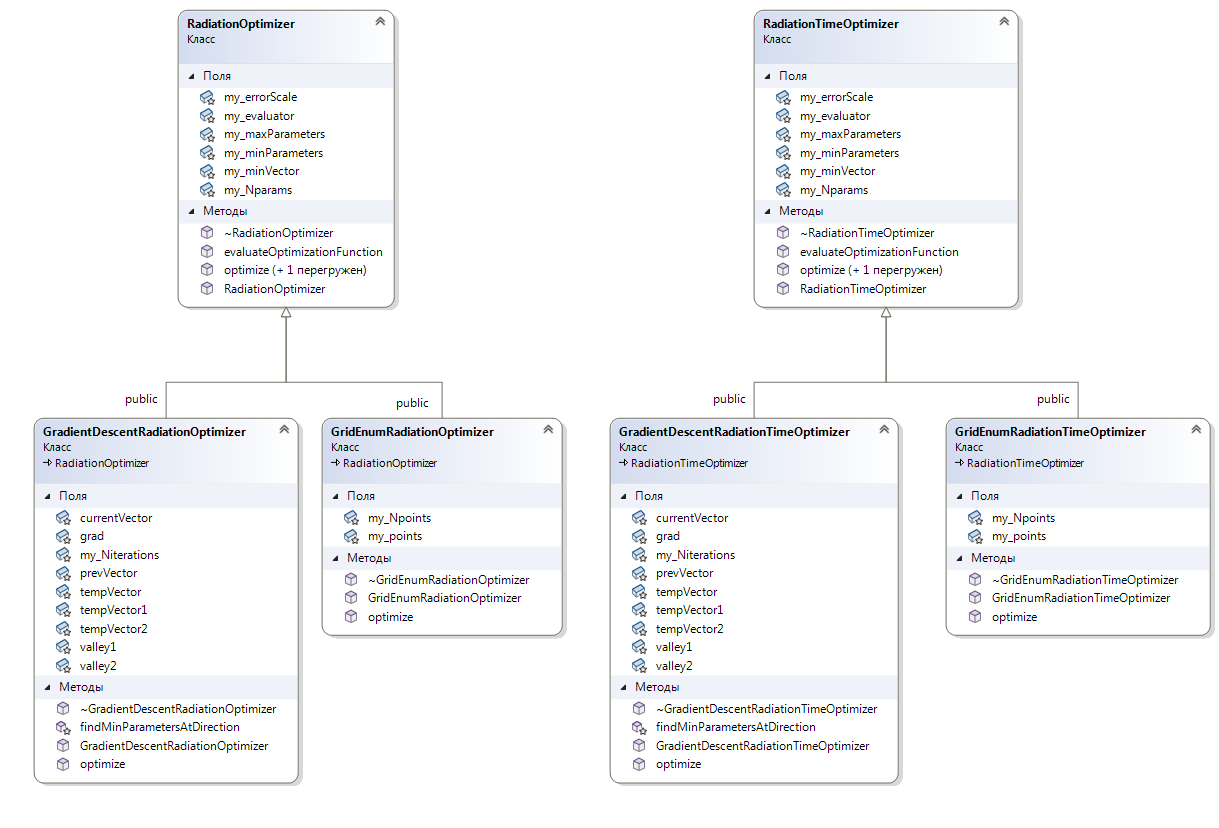
\includegraphics[width=11.5 cm]{./fig/radiationOptimizer.png} 
	\caption{Схема наследования классов оптимизаторов}
	\label{radiationOptimizer}
\end{figure}

\begin{small}
	\topcaption{Публичные методы классов оптимизаторов параметров источников }
	\label{RadiationOptimizerMethods}
	\begin{xtabular}{|p{0.41\textwidth}|p{0.59\textwidth}|}
		\hline
		\textbf{RadiationOptimizer} & абстрактный класс для оптимизации параметров источника \\
		\hline
		double evaluateOptimizationFunction(const double* vector) & вычисляет целевую функцию - взвешенную при данном векторе параметров\\
		\hline
		void optimize(double* vector, bool* optPar) & функция, осуществляющая оптимизацию, принимает на вход массив подбираемых параметров, в который будет записан результат и массив булевских переменных, определяющих оптимизировать соответствующий параметр, или считать его фиксированным\\
		\hline
		void outputProfileDiagrams(const double* vector, int Npoints) & функция, которая строит и записывает в файлы двухмерные сечения целевой функции по всем комбинациям параметров, проходящие через точку определяемую заданным вектором параметров\\
		\hline
		void outputOptimizedProfileDiagram(const double* vector, bool* optPar, int Npoints, int Nparam1, int Nparam2) & функция, которая строит и записывает в файлы двухмерные сечения целевой функции, в которых два параметра с номерами Nparam1 и Nparam2 фиксируются и пробегают соответствующую плоскость, а остальные оптимизируются\\
		\hline
		\textbf{GridEnumRadiationOptimizer} & класс предназначенный для оптимизации параметров с помощью перебора по сетке\\
		\hline
		GridEnumRadiationOptimizer(RadiationEvaluator* evaluator, const double* minParameters, const double* maxParameters, int Nparams, const int* Npoints, LossEvaluator* lossEvaluator) & конструктор, создает экземпляр класса с указанным вычислителем излучения, минимальными и максимальными значениями оптимизируемых параметров, количеством этих параметров, массивом с количеством перебираемых точек по каждому параметру и вычислителем целевой функции. При переборе точки будут распределены логарифмически по оси.\\
		\hline
		\textbf{GradientDescentRadiationOptimizer} & класс, предназначенный для оптимизации параметров методом градиентного спуска\\
		\hline
		GradientDescentRadiationOptimizer(RadiationEvaluator* evaluator, const double* minParameters, const double* maxParameters, int Nparams, int Niterations, LossEvaluator* lossEvaluator) & конструктор, создает экземпляр класса с указанным вычислителем излучения, минимальными и максимальными значеними оптимизируемых параметров, количеством этих параметров,  максимальным количеством итераций градиентного спуска и вычислителем целевой функции\\
		\hline
		\textbf{CombinedRadiationOptimizer} & класс, предназначенный для совместного использования сеточного поиска и градиентного спуска\\
		\hline
		CombinedRadiationOptimizer( RadiationEvaluator* evaluator, const double* minParameters, const double* maxParameters, int Nparams, int Niterations, const int* Npoints, LossEvaluator* lossEvaluator) & конструктор, создает экземпляр класса с указанным вычислителем излучения, минимальными и максимальными значеними оптимизируемых параметров, количеством этих параметров,  максимальным количеством итераций градиентного спуска, количеством точек для сеточного поиска и вычислителем целевой функции\\
		\hline
	\end{xtabular}
\end{small}

Пример фитирования параметров источника по наблюдательным данным приведен в функции fitCSS161010withPowerLawDistribition в файле examples.cpp. Следуя авторам работы \cite{Coppejans2020} произведем расчет синхротронного излучения источника с учетом самопоглощения, считая функцию распределения электронов чисто степенной с показателем 3.6. Но мы не будем накладывать дополнительную связь на параметры и предполагать равенство распределения энергии между магнитным полем и ускоренными частицами, вместо этого магнитное поле и концентрация электронов будут независимыми параметрами.

Подберем параметры Быстрого Оптического Голубого Транзиента CSS161010 на 98 день после вспышки на основе радиоизлучения. Зададим параметры источника на основе дынных статьи \cite{Coppejans2020}, которые будут использоваться в качестве начального приближения, а так же расстояние до него.
\begin{lstlisting}[language=c++]
    double electronConcentration = 25;
    double B = 0.6;
    double R = 1.4E17;
    double fraction = 0.5;
    const double distance = 150 * 1E6 * parsec;
\end{lstlisting}
Далее зададим степенное распределение электронов, с показателем 3.6 и источник в форме плоского диска, перпендикулярного лучу зрения, и вычислитель синхротронного излучения.
\begin{lstlisting}[language=c++]
    double Emin = me_c2;
    double Emax = 10000 * me_c2;
    double index = 3.6;
	
    SynchrotronEvaluator* synchrotronEvaluator = new
        SynchrotronEvaluator(200, Emin, Emax);

    MassiveParticlePowerLawDistribution* electrons = 
        new MassiveParticlePowerLawDistribution(
        massElectron, index, Emin, electronConcentration);

    SimpleFlatSource* source = new
        SimpleFlatSource(electrons, B, pi/2, R, fraction * R, distance);
\end{lstlisting}
Теперь определим вектор оптимизируемых параметров - это размер, магнитное поле, концентрация электронов и доля толщины, показывающая какю долю от радиуса диска составляет его толщина. И именно такие параметры ожидает функция resetParameters у источника SimpleFlatSource. Так же нужно указать минимальные и максимальные значения параметров, которые ограничат область поиска. Максимальные значения так же будут использоваться как константы нормировки.
\begin{lstlisting}[language=c++]
    const int Nparams = 4;
    double minParameters[Nparams] = { 1E17, 0.01, 0.5, 0.1 };
    double maxParameters[Nparams] = { 2E17, 10, 200, 1.0 };
    double vector[Nparams] = { R, B, electronConcentration, fraction};
    for (int i = 0; i < Nparams; ++i) {
	    vector[i] = vector[i] / maxParameters[i];
    }
\end{lstlisting}
Зададим наблюдательные данные, которые и будем фитировать. Обратите внимание, что частоты нужно перевести в энергии, а спектральную плотность потока - в энергетическую (в единицы $\text{см}^{-2}\text{с}^{-1}$).
\begin{lstlisting}[language=c++]
    const int Nenergy1 = 4;
    double energy1[Nenergy1] = { 1.5E9*hplank, 3.0E9 * hplank, 
    	6.1E9 * hplank, 9.8E9 * hplank };
    double observedFlux[Nenergy1] = { 1.5/(hplank*1E26), 
    	4.3/(hplank*1E26), 6.1/(hplank*1E26), 4.2 /(hplank*1E26)};
    double observedError[Nenergy1] = { 0.1 / (hplank * 1E26), 
    	0.2/(hplank*1E26), 0.3/(hplank*1E26), 0.2/(hplank*1E26)};
\end{lstlisting}
Далее создадим вычислитель целевой функции, фитирующий спектр и комбинированный оптимизатор, и укажем количество точек для перебора и количество итераци градиентного спуска. Так же укажем, что оптимизируем все параметры.
\begin{lstlisting}[language=c++]
    bool optPar[Nparams] = { true, true, true, true };
    int Niterations = 20;
    int Npoints[Nparams] = { 10,10,10,10 };
    
    LossEvaluator* lossEvaluator = new SpectrumLossEvaluator(energy1, observedFlux, observedError, Nenergy1, source);
    RadiationOptimizer* optimizer = new CombinedRadiationOptimizer(
        synchrotronEvaluator,minParameters,maxParameters,Nparams, Niterations,Npoints, lossEvaluator);
\end{lstlisting}
Применим функцию optimize и изменим параметры источника на оптимальные
\begin{lstlisting}[language=c++]
    optimizer->optimize(vector, optPar, energy1, observedFlux, 
        observedError, Nenergy1, source);
    source->resetParameters(vector, maxParameters);
\end{lstlisting}
Полученные в результате оптимизации парметры источника равны: радиус диска $R = 1.8\times10^17 \text{ см}$, магнитное поле $B = 1.6 \text{ Гс}$, концентрация электронов $n = 2.3 \text{ см}^{-3}$, доля толщины $fraction = 0.54 $. Значение целевой функции $f \approx 50$. Модельный спектр излучения  с данными параметрами и наблюдательные данные изображены на рисунке \ref{synchrotron1}.
\begin{figure}[h]
	\centering
	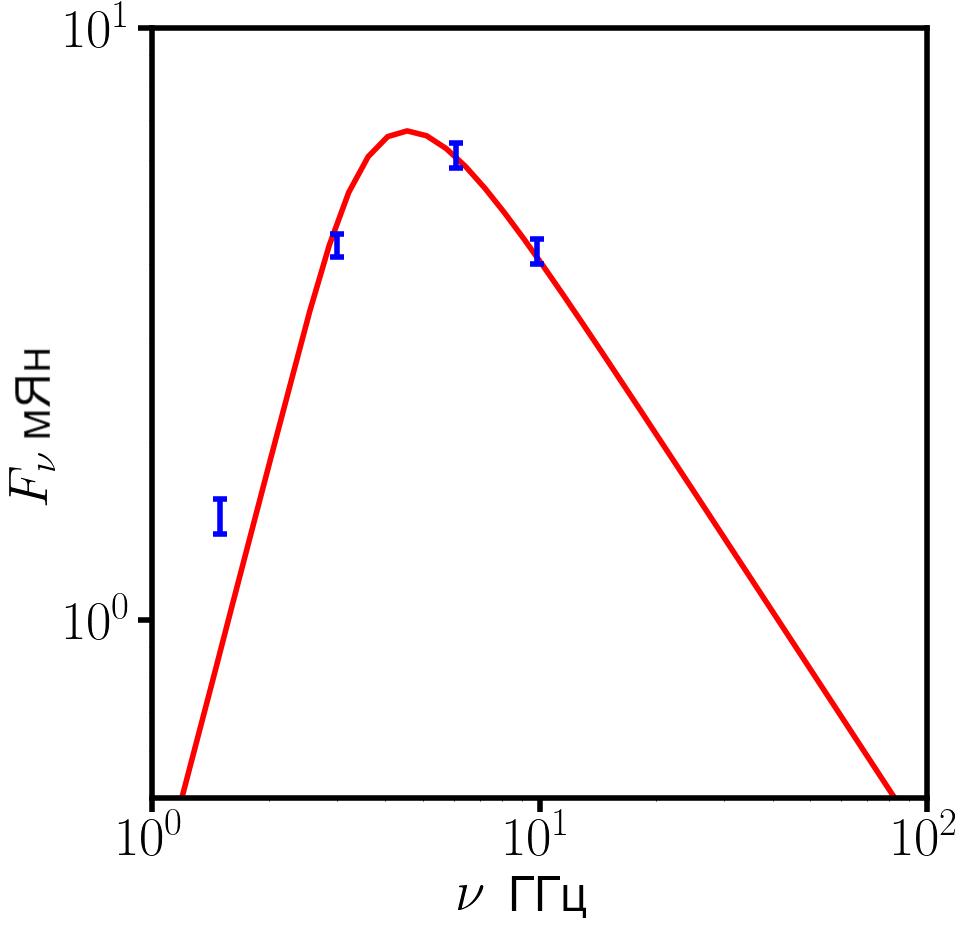
\includegraphics[width=12.5 cm]{./fig/synchrotron1.png} 
	\caption{Наблюдаемый и расчетный спектр радиоизлучения объекта CSS161010 на 98 день после вспышки}
	\label{synchrotron1}
\end{figure}


%Пример фитирования параметров источника по наблюдательным данным приведен в функции fitTimeDependentCSS161010() в файле examples.cpp. Подберем параметры Быстрого Оптического Голубого Транзиента CSS161010 на основе наблюдений радиоизлучения, проведенных на 98, 162, 357 день после вспышки.  Расчет синхротронного излучения учитывает самопоглощение и раширение источника. Источник будем считать шаровым слоем с однородной плотностью и однороным магнитным полем, направленным перпендикулярно лучу зрения. Функцию распределения излучающих электронов возьмем на основе Particle-in-Cell расчетов для ударной волны со скоростью 0.3c,как сделано в работе \cite{BykovUniverse}. Учтена зависимость функции распределения от угла между магнитным полем и направлением распространения ударной волны.

%Подберем параметры Быстрого Оптического Голубого Транзиента CSS161010 на основе наблюдений радиоизлучения, проведенных на 98, 162, 357 день после вспышки.  Зададим сначала массивы наблюдательных точек, переведя при этом из единиц герцы и милиянские в эрги и $\text{см}^{-2} \text{c}^{-1}$
%\begin{lstlisting}[language=c++]
%const double cssx1[4] = 
%{1.5*hplank*1E9, 3.0*hplank*1E9, 6.1*hplank*1E9, %9.87*hplank*1E9};
%const double cssy1[4] =  {1.5/(hplank*1E26), 
%4.3/(hplank*1E26), 6.1/(hplank*1E26), 4.2/(hplank*1E26)};
%const double cssError1[4] = {0.1/(hplank*1E26), 
%0.2/(hplank*1E26), 0.3/(hplank*1E26), 0.2/(hplank*1E26)};
	
%const double cssx2[4] = 
%{2.94*hplank*1E9, 6.1*hplank*1E9, 9.74*hplank*1E9, %22.0*hplank*1E9};
%const double cssy2[4] = {2.9/(hplank*1E26), 
%2.3/(hplank*1E26), 1.74/(hplank*1E26), %0.56/(hplank*1E26)};
%const double cssError2[4] = {0.2/(hplank*1E26), 
%0.1/(hplank*1E26), 0.09/(hplank*1E26), %0.03/(hplank*1E26)};
	
%const double cssx3[6] = {0.33*hplank*1E9, %0.61*hplank*1E9, 
%1.5*hplank*1E9, 3.0*hplank*1E9, 6.05*hplank*1E9, %10.0*hplank*1E9};
%const double cssy3[6] = {0.375/(hplank*1E26), %0.79/(hplank*1E26), 
%0.27/(hplank*1E26),0.17/(hplank*1E26),0.07/(hplank*1E26),0.32/(hplank*1E27)};
%const double cssError3[6] = {0.375/(hplank*1E26), 0.09/(hplank*1E26),
%0.07/(hplank*1E26),0.03/(hplank*1E26),0.01/(hplank*1E26),0.8/(hplank * 1E28)};
%\end{lstlisting}

%Определим моменты времени инаблюдений и соответствующие им количества точек

%\begin{lstlisting}[language=c++]
%const int Ntimes = 3;
%double times[Ntimes] = { 99 * 24 * 3600, 162 * 24 * 3600, 357 * 24 * 3600 };
%int Nenergy[Ntimes];
%Nenergy[0] = 4;
%Nenergy[1] = 4;
%Nenergy[2] = 6;
%\end{lstlisting}
%Создадим и инициализируем необходимые массивы с наблюдательными данными
%\begin{lstlisting}[language=c++]
%double** energy = new double* [Ntimes];
%double** F = new double* [Ntimes];
%double** Error = new double* [Ntimes];
%for (int m = 0; m < Ntimes; ++m) {
%	energy[m] = new double[Nenergy[m]];
%	F[m] = new double[Nenergy[m]];
%	Error[m] = new double[Nenergy[m]];
%}

%for (int i = 0; i < Nenergy[0]; ++i) {
%	energy[0][i] = cssx1[i];
%	F[0][i] = cssy1[i];
%	Error[0][i] = cssError1[i];
%}

%for (int i = 0; i < Nenergy[1]; ++i) {
%	energy[1][i] = cssx2[i];
%	F[1][i] = cssy2[i];
%	Error[1][i] = cssError2[i];
%}

%for (int i = 0; i < Nenergy[2]; ++i) {
%	energy[2][i] = cssx3[i];
%	F[2][i] = cssy3[i];
%	Error[2][i] = cssError3[i];
%}
%\end{lstlisting}

%Зададим физические параметры источника (или их начальные приближения) - расстояние, размер, концентрацию, магнитное поле, долю толщины шара, занятую излучающим веществом, скорость расширения и магнетизацию.

%\begin{lstlisting}[language=c++]
%const double distance = 150 * 1E6 * parsec;
%double rmax = 1.3E17;
%double electronConcentration = 150;
%double B = 0.6;
%double widthFraction = 0.5;
%double v = 0.3 * speed_of_light;
%double sigma = B * B / (4 * pi * massProton * 
%electronConcentration * speed_of_light2);
%\end{lstlisting}

%Укажем для оптимизаторов количество параметров, ихи минимальные и максимальные значения и соответствие вектора параметров и физических величин. Оптимизируемыми параметрами являются - размер источника, магнетизация, доля заполнения и скорость расширения в первый момент времени, а так же показатели степени расширения со временем и изменения магнитного поля и концентрации с радиусом, то есть $\alpha, \beta, \gamma$ где эти величины определены через уравнения $R(t) = R_0 + \frac{1}{\alpha-1}\cdot V(0) \cdot t_0 \cdot ({t/t_0}^{\alpha-1}-1 )$, $B(R) = B(R_0)\cdot{R_0/R}^{\beta-1}$, $n(R) = n(R_0)\cdot{R_0/R}^{\gamma - 1}$. Единица добавлена к показателям степени для удобства численных расчетов при близости величин к нулю.
%\begin{lstlisting}[language=c++]
%const int Nparams = 8;
%double minParameters[Nparams] = { 1E16, 0.0001, 0.01, 0.1, 
%0.01 * speed_of_light, 1.1, 1.0, 1.0 };
%double maxParameters[Nparams] = { 2E17, 1, 1000, 1.0, 0.6 * 
%speed_of_light, 2.0, 3.5, 3.5 };
%double vector[Nparams] = { rmax, sigma, electronConcentration, 
%widthFraction, v, 2.0, 2.0, 3.0 };
%for (int i = 0; i < Nparams; ++i) {
%    vector[i] = vector[i] / maxParameters[i];
%}
%bool optPar[Nparams] = { true, true, true, true, true, %true, true, true };
%\end{lstlisting}

%Далее создадим источник излучения. Воспользуемся моделью расширяющейся однородной сферической оболочки, с однородным магнитным полем, перпендикулярным лучу зрения и функцией распределения электронов, зависящей от угла между направлением магнитного поля и направлением расширения оболочки. Функции распределения получены с использованием Particle-in-Cell кода Smilei \cite{Derouillat} и содержатся в директории examplesData. Методика расчетов описана в статье \cite{BykovUnirse}. Количетсво распределений, посчитанных для углов от 0 до 90 градусов равно десяти. Их можно считать из соответствующих файлов, используя метод класса MassiveParticleDistributionFactory. Так же будет добавлено продолжение мтепенного хвоста, так как PIC расчеты не пользволяют получать длинные спектры из-за большой вычислительной сложности. Так же необходимо провести масштабирование распределения, так как в PIC расчетах испольовалось уменьшенное отношение масс протонов и электронов $m_p/m_e = 100$. Имея массив распределений создадим источник, учитывающий угловую зависимость, и передим его далее источнику. учитывающему зависимость от времени.

%\begin{lstlisting}[language=c++]
%const int Ndistributions = 10;

%MassiveParticleIsotropicDistribution** angleDependentDistributions = 
%MassiveParticleDistributionFactory::readTabulatedIsotropicDistributionsAddPowerLawTail
%(massElectron, "./input/Ee", "./input/Fs", ".dat", 10, 
%DistributionInputType::GAMMA_KIN_FGAMMA, electronConcentration, 200, 20 * me_c2, 3.5);
%for (int i = 0; i < Ndistributions; ++i) {
%(dynamic_cast<MassiveParticleTabulatedIsotropicDistribution*>
%(angleDependentDistributions[i]))->rescaleDistribution(sqrt(18));
%}

%AngleDependentElectronsSphericalSource* angleDependentSource = new 
%AngleDependentElectronsSphericalSource(20, 20, 4, Ndistributions, 
%angleDependentDistributions,B,1.0,0,electronConcentration,rmax,0.5*rmax,distance);

%RadiationTimeDependentSource* source = new 
%ExpandingRemnantSource(rmax, B, electronConcentration, 0.3 * speed_of_light,
%0.5, angleDependentSource, times[0]);

%\end{lstlisting}

%Теперь создадим вычислитель синхротронного излучения и два оптимизатора параметров - первый будет работать перебором параметров по сетке, а второй - градиентным спуском. Укажем количество точек по осям для перебора, количество итераций для градиентного спуска и диапазон энергий электронов, который будет рассматривать вычислитель синхротронного излучения.

%\begin{lstlisting}[language=c++]
%int Npoints[Nparams] = { 3, 3, 3, 3, 3, 3, 3, 3 };
%int Niterations = 5;

%double Emin = me_c2;
%double Emax = 10000 * me_c2;

%SynchrotronEvaluator* synchrotronEvaluator=new %SynchrotronEvaluator(200, Emin, Emax);

%RadiationTimeOptimizer* gridEnumOptimizer = 
%new GridEnumRadiationTimeOptimizer(synchrotronEvaluator, minParameters, 
%maxParameters, Nparams, Npoints);
%RadiationTimeOptimizer* gradientOptimizer = 
%new GradientDescentRadiationTimeOptimizer(synchrotronEvaluator,minParameters, 
%maxParameters, Nparams, Niterations);
%\end{lstlisting}

%Применим созданые оптимизаторы и изменим параметры источника на найденные, соответствующие минимуму.

%\begin{lstlisting}[language=c++]

%gridEnumOptimizer->optimize(vector, optPar, energy, F, Error, Nenergy, Ntimes, times, source);

%gradientOptimizer->optimize(vector, optPar, energy, F, Error, Nenergy, Ntimes, times, source);

%source->resetParameters(vector, maxParameters);
%\end{lstlisting}

%Полученные в результате оптимизации парметры источника равны: радиус диска в начальный момент времени $R = 1.8\times10^17 \text{ см}$, магнитное поле $B = 1.6 \text{ Гс}$, концентрация электронов $n = 2.3 \text{ см}^{-3}$, доля толщины $fraction = 0.54 $, степени зависимости . Значение целевой функции $f \approx 50$. Модельный спектр излучения  с данными параметрами и наблюдательные данные изображены на рисунке \ref{synchrotronSeries}.

%\begin{figure}
%	\centering
%	%\includegraphics[width=12.5 cm]{./fig/synchrotronSeries.png} 
%	\caption{Наблюдаемый и расчетный спектр радиоизлучения объекта CSS161010 на 99, 162 и 357 дни после вспышки}
%	\label{synchrotronSeries}
%\end{figure}